\documentclass[a4paper]{article}

\usepackage[czech]{babel} %https://github.com/michal-h21/biblatex-iso690
\usepackage[
   backend=biber      % if we want unicode 
  ,style=iso-numeric % or iso-numeric for numeric citation method          
  ,babel=other        % to support multiple languages in bibliography
  ,sortlocale=cs_CZ   % locale of main language, it is for sorting
  ,bibencoding=UTF8   % this is necessary only if bibliography file is in different encoding than main document
]{biblatex}

\usepackage{mathtools}
\usepackage[utf8]{inputenc}
\usepackage{fancyhdr}
\usepackage{amsmath}
\usepackage{amssymb}
\usepackage[left=2cm,right=2cm,top=2.5cm,bottom=2.5cm]{geometry}
\usepackage{graphicx}
\usepackage{pdfpages}
\usepackage{url}
\usepackage{multirow}

\usepackage{siunitx}
\sisetup{locale = DE, separate-uncertainty = true} %    kdybych chtel +/-

\usepackage{float}
\newfloat{graph}{htbp}{grp}
\floatname{graph}{Graf}
\newfloat{tabulka}{htbp}{tbl}
\floatname{tabulka}{Tabulka}

\renewcommand{\thefootnote}{\roman{footnote}}

\pagestyle{fancy}
\lhead{Praktikum IV - (A18) Určení strukturních parametrů krystalických látek\\ metodami elektronové mikroskopie (SEM)}
\rhead{Vladislav Wohlrath}
\author{Vladislav Wohlrath}

\bibliography{source}

\begin{document}

\begin{titlepage}
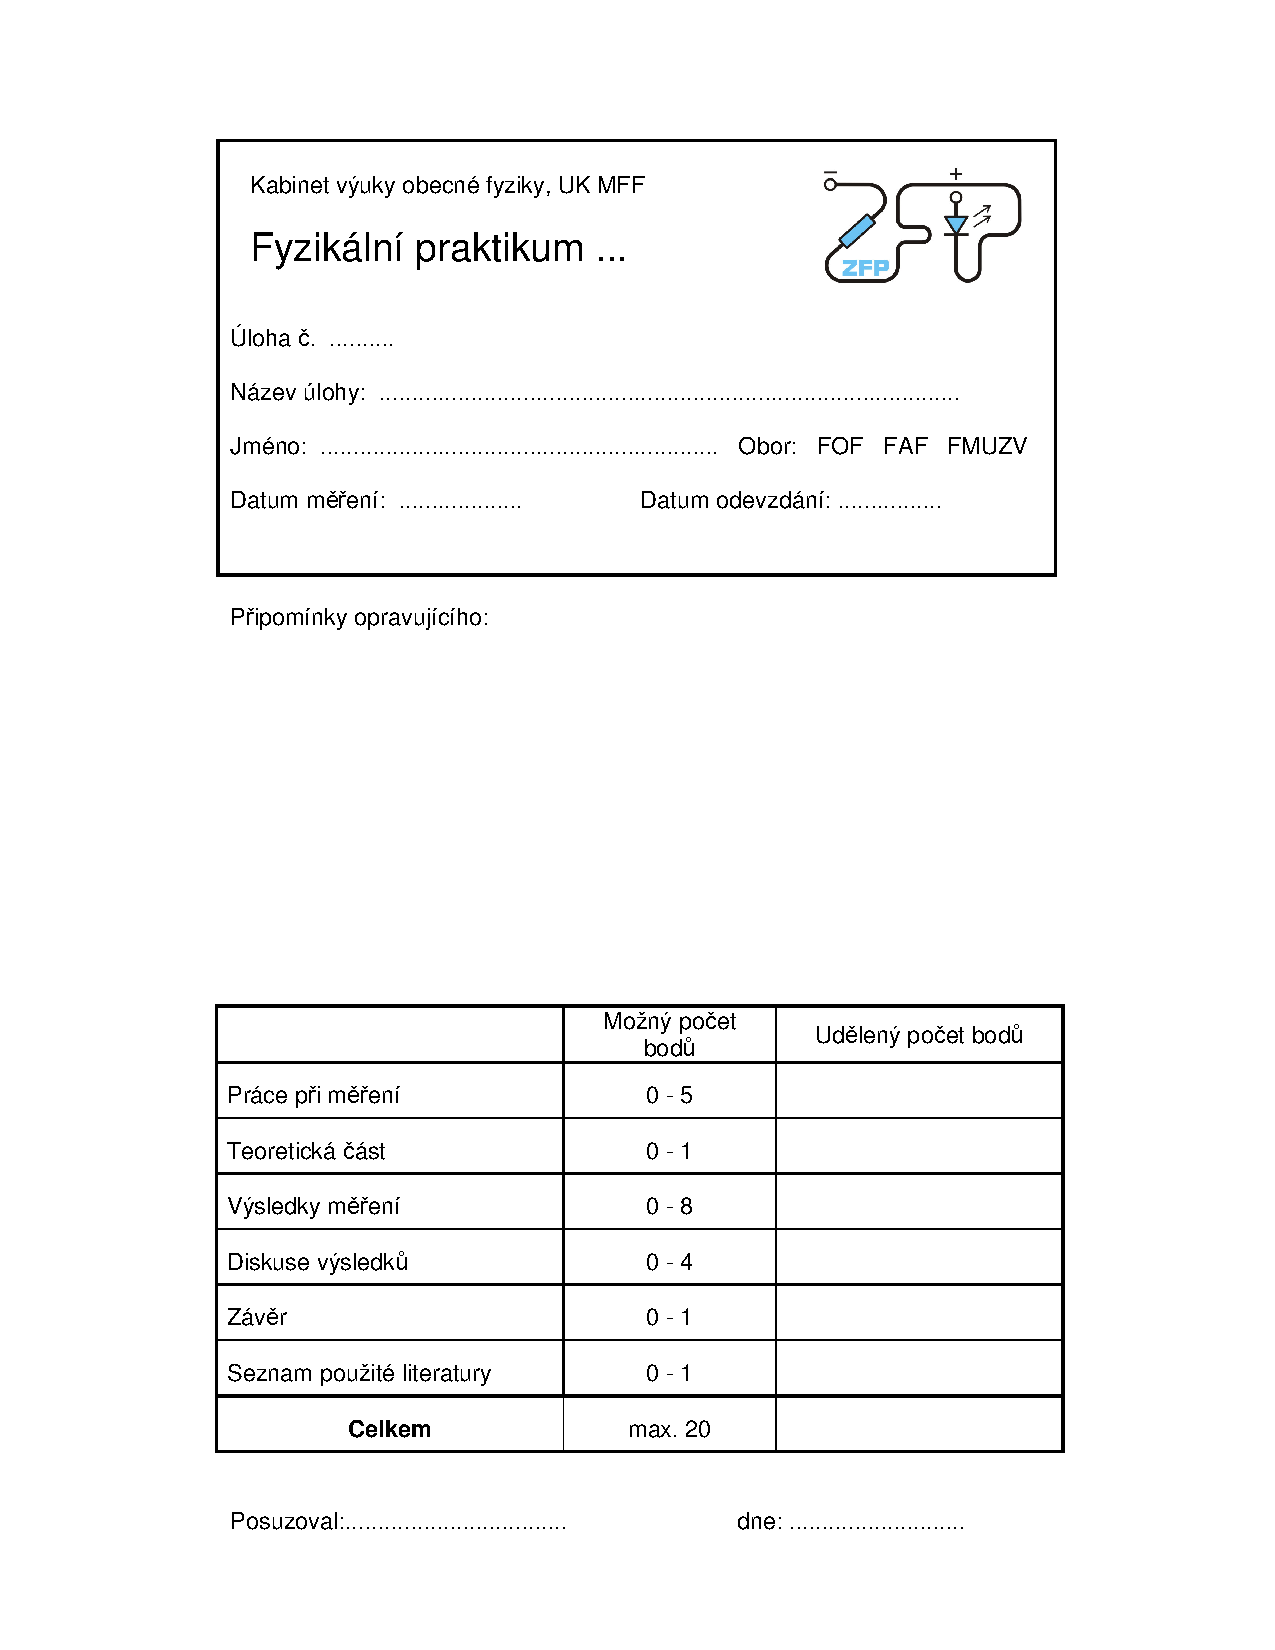
\includepdf[pages={1}]{./graficos/titlelist.pdf}
\end{titlepage}

\section*{Pracovní úkoly}
\begin{enumerate}
\item Studium lomových ploch pomocí SEM.
\item Měření střední velikosti zrna polykrystalického vzorku. K vyhodnocení snímku ze scanovacího elektronového mikroskopu použijte kruhovou metodu.
\item Určení frakčního objemu dané fáze ve vícefázovém materiálu. Použijte specializované programové vybavení pro obrazovou analýzu.
\end{enumerate}

%Teoretická část
\section*{Teoretická část}
Skenovací elektronový mikroskop je přístroj, který pomocí fokusovaného svazku primárních elektronů postupně vytváří zvětšený obraz vzorku bod po bodu. Po dopadu na vzorek může nastat několik druhů událostí, jejichž detekce nám může poskytnout informaci o povrchu vzorku, my se zaměříme na dva z nich.

Elektron se může pružně odrazit zpět (BSE). Intenzita zpětně odražených elektronů je mimo jiné závislá na protonovém čísle (takže nám umožňuje pozorovat chemické složení vzorku) a na orientaci krystalografických rovin (tzv. channelling).

Elektron také může z atomů vzorku vyrazit sekundární elektron (SE). Tímto způsobem můžeme pozorovat topografii vzorku.

Pokud máme mikroskopický snímek zrnitého vzorku, můžeme z něj určit střední velikost zrna kruhovou metodou \cite{skripta}. Narýsujeme kružnici o průměru $D$ a spočítáme počet zrn, které protne. Tento počet označíme $n$. Potom střední velikost zrn $d$ je dána vztahem \cite{skripta}
\begin{equation} \label{e:kruhy}
d=\frac{3\pi}{2} \frac{D}{n} \,,
\end{equation}
kde $\pi$ je Ludolfovo číslo.

%Výsledky měření
\section*{Výsledky měření}

%Diskuze výsledků
\section*{Diskuze}

%Závěr
\section*{Závěr}


\printbibliography[title={Seznam použité literatury}]

\end{document}